\documentclass{article}
\usepackage{graphicx}
\usepackage{float}
\usepackage[utf8]{inputenc}

\begin{document}

\title{\vspace{-0.0in}\hspace{+0.5in}18.s096 - Final Project \\
Applications of PCA in Finance}
\author{Dimitris Koutentakis}
\date{}


\maketitle


%\addtolength{\oddsidemargin}{-0.0in}

\textbf{ Abstract} 
\vspace{2mm}

In this paper, I discuss the application of Principal Component Analysis (PCA) in the financial domain, and specifically in portfolio management. I apply PCA to time series of financial data (9 of the top Tech stocks by market value from 2015 until today) in order to optimize portfolio investments. I conclude that PCA is robust and is likely to produce stable portfolio returns.

\section{Introduction}
The aim of Principal Component Analysis (PCA) is to in a particular way simplify data containing a lot of interrelated variables. In a broad sense, it means finding linear combinations of the variables that account for most of the data's variation, in order to simplify the analysis all while preserving the data's original variation as much as possible. This method reduces the complexity of analysis, as the data is made into a linear model, with fewer dimensions.

PCA involves applying a transformation to the data in order to obtain what we call the uncorrelated principle components- which, when ordered, will contain, in the first few, as much as possible of the original variables' variations. The number of components needed to capture most of the data's variance will depend on data and its structure.

More mathematically, and a part of which we will show in the proof at the crux of this paper, PCA is an orthogonal linear transformation transforming (or rotating in respect to the data mean) the data to a new coordinate system. 
The first resulting principle component, corresponding to the first greatest variance, will also correspond to the first coordinate, and so on with the descending variances corresponding to following appropriately ranked coordinates.

It is important to note that before applying PCA, the data in question should be prepared. The goal is to get the data as close to following a multivariate normal distribution as possible. That is because data that follows a multivariate normal distribution is fully parametrized by its mean and covariance matrix. In particular, preparing the data for PCA involves centering the data by its mean, or "demeaning" it. This ensures that the orthogonal linear transformation of PCA, the rotation in respect to the data mean, is truly centered.

PCA is widely used in data science- for example, in face recognition, compression or in finance, which we will touch upon later in this paper with our example illustration of PCA.

In a geometric sense, the first of the ordered principal components will be a line through $(0,0)$ closest to all the points in a perpendicular direction. In contrast with Ordinary Least Squares (OLS), PCA solves a perpendicular least squares optimization, or orthogonal regression. Regular regression, or OLS minimizes the vertical distance to the points, as seen in Figure \ref{pca_vs_regression}.


\begin{figure}[!hpt]
    \caption{Red: OLS, Blue: PCA}
    \centering
    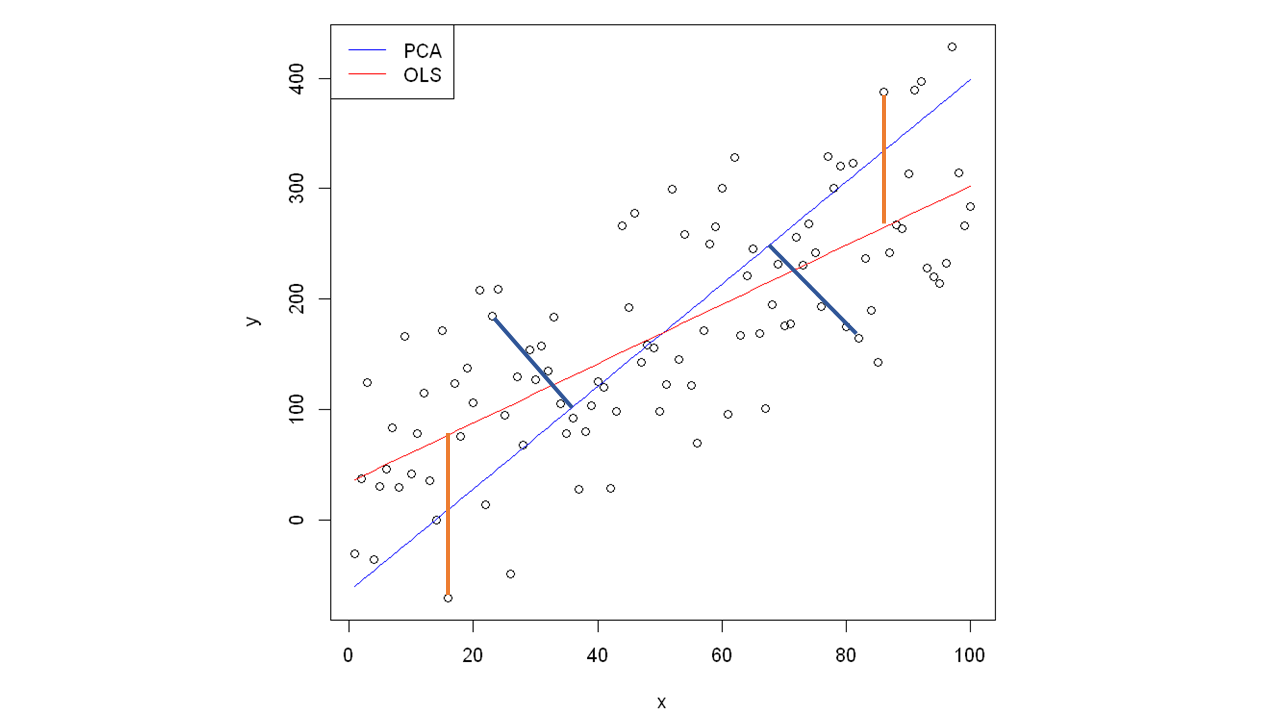
\includegraphics[width=0.8\textwidth]{pcavsols.png}
    \label{pca_vs_regression}
\end{figure}


\section{Proof}

In this section, we provide a quick derivation of PCA. Essentially, we will show how to acquire the maximum variance of the data in question, a key aspect of PCA. We start with the following matrices:\\
\begin{itemize}
\item $P$, which has dimensions $n$ x $T$, is the matrix of prices.\\
Specifically, $P_{[i][j]}$ represents the price of the $i^{th}$ asset at time $j$ for $i\in[1,n]\ and\ j\in[1,T]$.\\
\item $R$, which has dimensions $n$ x $(T-1)$, is the matrix of specific returns (difference of prices divided by the initial price).\\
Specifically, $R_{[i][j]} = (P_{[i][j+1]} - P_{[i][j]})/P_{[i][j]}\ for \ i\in[1,n]\ and\ j\in[1,T-1]$.\\
\end{itemize}
We begin by centering each of the entries of $R$ by the mean of each row.\\ We introduce
$\overline{R}$, which has dimensions $n$ x $1$, and is the matrix of means of rows such that 
$$\overline{R}_{[i]} = \frac{1}{T-1} \sum_{k=1}^{T-1} R_{[i][k]}.$$
Additionally, let $X = R - \overline{R}$.\\
We define the covariance matrix $\Sigma = \frac{1}{T-2}(XX^T)$.\\
Let $u_k$ be an $n$ x $1$ vector such that $u_k$ is the $k^{th}$ principal component of $X$. By definition, the variance of our data matrix is maximized along the $k^{th}$ principal component. The variance of $X$ along the $k^{th}$ principal component is found as follows:
$$Var(X^{T}u_k) = u_{k}^{T}XX^{T}u_k = (T-2)u_{k}^{T}\Sigma u_k.$$
Our goal is to maximize $Var(X^{T}u_k)$ by choosing $u_k$ that maximizes the variance up to a constant multiplier.\\
Let $k=1$. Then, we have a setup for a constrained optimization problem which consists of maximizing the variance $Var(X^{T}u_1)$ under the constraint $\vert\vert u_{1} \vert\vert = 1$. Using Lagrange multipliers (denoted as $\lambda_{1}$), we get:\\
$$\max_{(\lambda_{1},u_{1})}u_{1}^{T}\Sigma^{T}u_{1}-\lambda_{1}(u_{1}^{T}u_{1}-1)$$
$$\frac{\partial}{\partial u_1}(u_{1}^{T}\Sigma u_1-\lambda_{1}(u_{1}^{T}u_{1}-1))=0=\Sigma u_1 - \lambda_1 u_1 $$ so
$$\Sigma u_1 = \lambda_{1}u_1 .$$
The last equations suggests that 
$u_1$ is an eigenvector of $\Sigma$ with eigenvalue $\lambda_1$.\\ We also have that, 
$$Var(X^{T}u_1)=(T-2)u_{1}^{T}\Sigma u_1=(T-2)u_{1}^{T}\lambda_{1}u_{1}=(T-2)\lambda_1.$$
Therefore, to maximize the variance, we maximize $\lambda_1 $ which translates to choosing  the eigenvector corresponding to the largest eigenvalue of $\Sigma$.
\\
We are now going to compute the second principal component. Let $k=2$. Then, we have a setup for a constrained optimization problem which consists of maximizing the variance $Var(X^{T}u_2)$ under the constraints $\vert\vert u_{2} \vert\vert = 1$ and $u_2 \perp u_1$. Using Lagrange multipliers (denoted as $\lambda_{2}$ and $\lambda_{3}$), we get the following optimization problem:\\


$$\max_{(\lambda_{2}, \lambda_{3},u_{2})}u_{2}^{T}\Sigma^{T}u_{2}-\lambda_{2}(u_{2}^{T}u_{2}-1) - \lambda_{3} u_2^T u_1$$
$$\frac{\partial}{\partial u_2}(u_{2}^{T}\Sigma^{T}u_{2}-\lambda_{2}(u_{2}^{T}u_{2}-1) - \lambda_3 u_2^T u_1)=0=\Sigma u_2 - \lambda_2 u_2 - \lambda_3 u_1 .$$
By multiplying the equation above by $u_1^T$ to the left, we get:

$$
u_1^T \Sigma u_2  -  \lambda_2 u_1^T u_2 - \lambda_3 \vert\vert u_1 \vert\vert^2 = 0
$$
Then, using orthogonality of $u_1$ and $u_2$, we find:
$$\lambda_3 \vert\vert u_1 \vert\vert^2 = 0 \ so\ \lambda_3 = 0.$$

We have found that the second Lagrange multiplier is equal to 0. This means that our optimization problem reduces to \\
$$\Sigma u_2 = \lambda_{2}u_2.$$
The last equations suggests that $u_2$ is an eigenvector of $\Sigma$ with eigenvalue $\lambda_2$.\\ We write, 
$$Var(X^{T}u_2)=(T-2)u_{2}^{T}\Sigma u_2=(T-2)u_{2}^{T}\lambda_{2}u_{2}=(T-2)\lambda_2.$$
Therefore, to maximize the variance, we maximize $\lambda_2 $ which translates to choosing  the eigenvector corresponding to the second largest eigenvalue of $\Sigma$.
It can be shown in the same manner that the $i^{th}$ principal component of matrix $X$ corresponds to the eigenvector of the $i^{th}$ biggest eigenvalue of the matrix $\Sigma$.






\section{Quantitative Application of Principal Component Analysis}

\subsection{DataSet}

In order to perform a PCA analysis on real stock trading data, we chose some of the top technology company stocks in the US. The stocks chosen are: Apple, Google, Microsoft, Facebook, Intel, Cisco, Nvidia, IBM and Qualcomm. The analysis was done in the language R, and the data was imported from the Yahoo Finance database using the package \texttt{quantmod}. The period we used to analyze the data was from January $1^{st}$ 2015 to May $1^{st}$ 2018. The data is summarized in figure \ref{fig:stockprices}.
\begin{figure}[!ht]
\caption{Stock Prices}
\centering
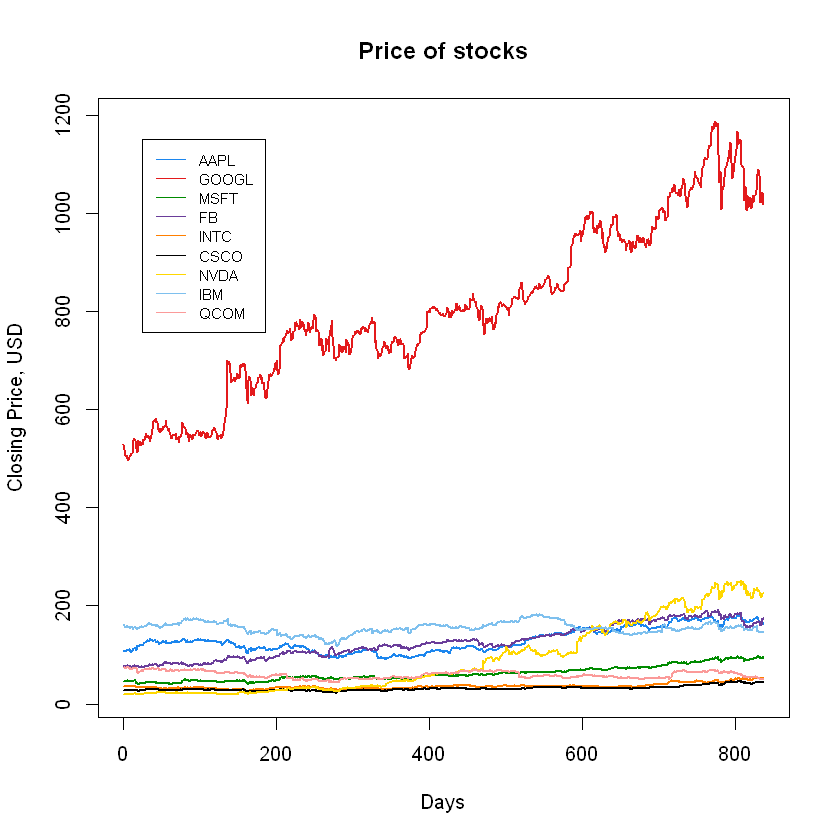
\includegraphics[width=0.75\textwidth]{stock_prices.png}
\label{fig:stockprices}
\end{figure}


\subsection{Data Preparation}
Our original data matrix $A'''$ has entries in the following form: the $A'''[i,j]$ entry has the price of the $i^{th}$ stock on the closing of the $j^{th}$  of T days. In order for the Principal Component Analysis to return meaningful results, we first have to prepare the data. This includes the following simple steps:
\begin{enumerate}
\item Convert prices to price differences:
$A''$ will have entries such that: $A''[i,j] = A'''[i, j+1]-A'''[i,j]$
\item Convert price differences to returns: 
$A'$ will have entries such that: $A'[i,j] = \frac{A''[i,j]}{A'''[i,j]}$
\item Demean the data: 
$A$ will have entries such that $A[i,j] = A'[i,j]-\frac{1}{T-2}\sum_{k=1}^{T-1}A'[i,k]$
\end{enumerate}
Following the data preparation, we find the covariance matrix as $\Sigma = \frac{AA^t}{T-2}$. Finally we find the eigenvalues and eigenvectors of $\Sigma$ ($u, \sigma, v$) so that in the end: $A = \Sigma_{i=1}^{T-1}u_i\sigma_iv_i^T$. Each of the principal components $PC_i = u_i^T A$ will explain $\frac{\lambda_i}{\Sigma_j\lambda_j}$ of the total variance (here and further, we use notation PC1, PC2, etc for principal components).

\subsection{Results}
Based on the analysis performed, we found that the first principal component explains almost half of the total variance, the second one around 15\% and the third one around 11\%, as can be seen in figure \ref{techvar_exp}.  

 
\begin{figure}[H]
\centering
\caption{}
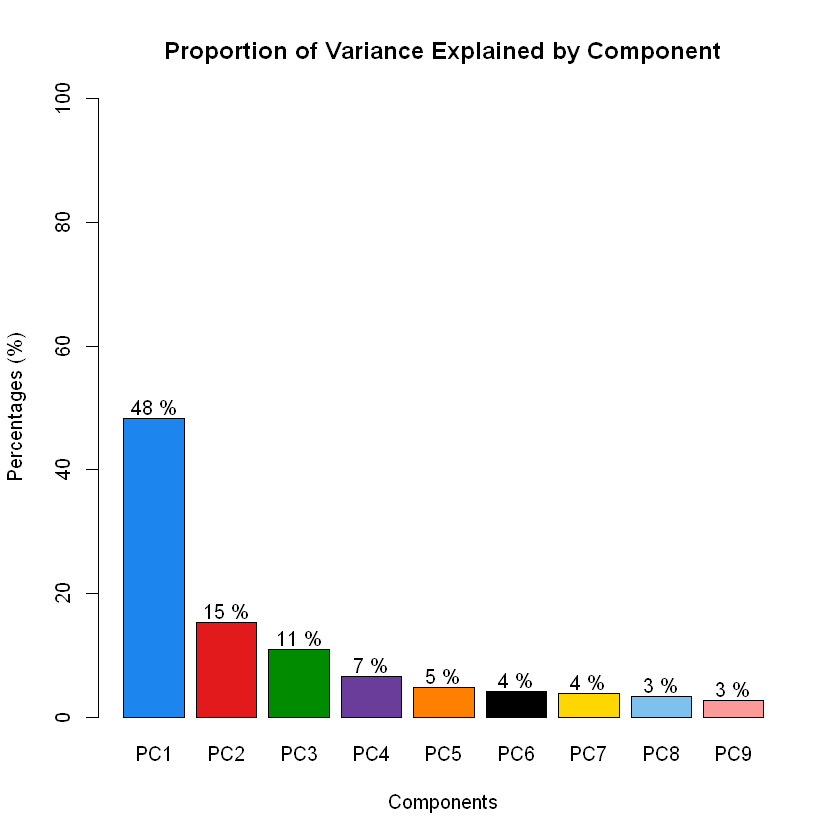
\includegraphics[width=0.75\textwidth]{allvar_exp.png}
\label{techvar_exp}
\end{figure}
This implies that the stocks of technology companies are not entirely independent, but also do not exhibit absolute dependency on one another. It also makes sense that the variance explanation is not very skewed towards PC1, as our time frame was long and in the fast-paced technology industry there are many changes. It would thus be unlikely to find one component that can explain very large amounts of variance for the whole of our time frame. 

This fact becomes even more obvious when looking at the graphs of loadings of principal components, essentially, coordinates of PC1, PC2, and PC3 (Fig. \ref{techloadings}).

\begin{figure}[!ht]
\caption{}
\centering
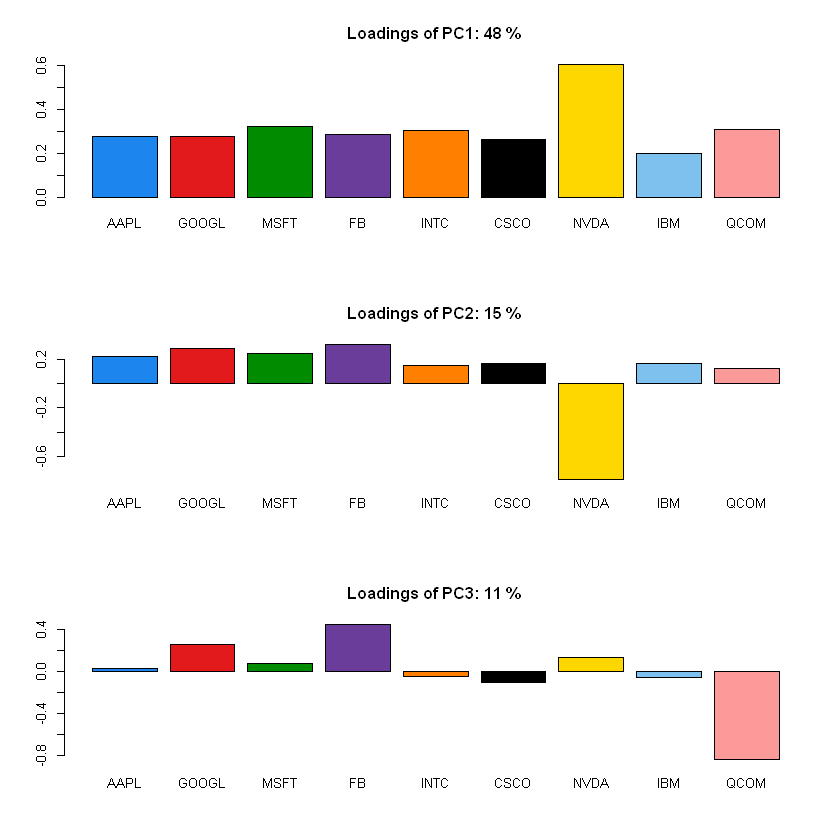
\includegraphics[width=0.75\textwidth]{PCload.png}
\label{techloadings}
\end{figure}


We can see that for the first principal component, all of the coordinates have similar values, thus PC1 explains the general trend of the tech industry.  The fact that the  $u$ vector corresponding to PC2 has the NVIDIA coefficient as the only negative, tells us that the convolution of $u_2$ with data will tell us the behavior of NVIDIA returns as compared with respect to the other companies. This fact suggested that NVIDIA returns were "the most unstable" in some sense over the period considered. On the other hand, since all coefficients are positive and lie approximately in the same range, we can say that market as a whole moves together at the majority of days. Finally, PC3 is similar in the sense that it explains how the rest of the stocks are doing compared to Qualcomm.



\subsection{Stability of PCA}

We can get a sense of how stable our analysis is by applying a rolling "window" principal component analysis. For that we take a k-month subsection of our data and apply PCA, then we move the window by one day and apply it again. By plotting the percentage of variance explained by each principal component, as well as the loadings of each vector, we can determine how robust our analysis is. 
\begin{figure}[H]
\caption{}
\centering
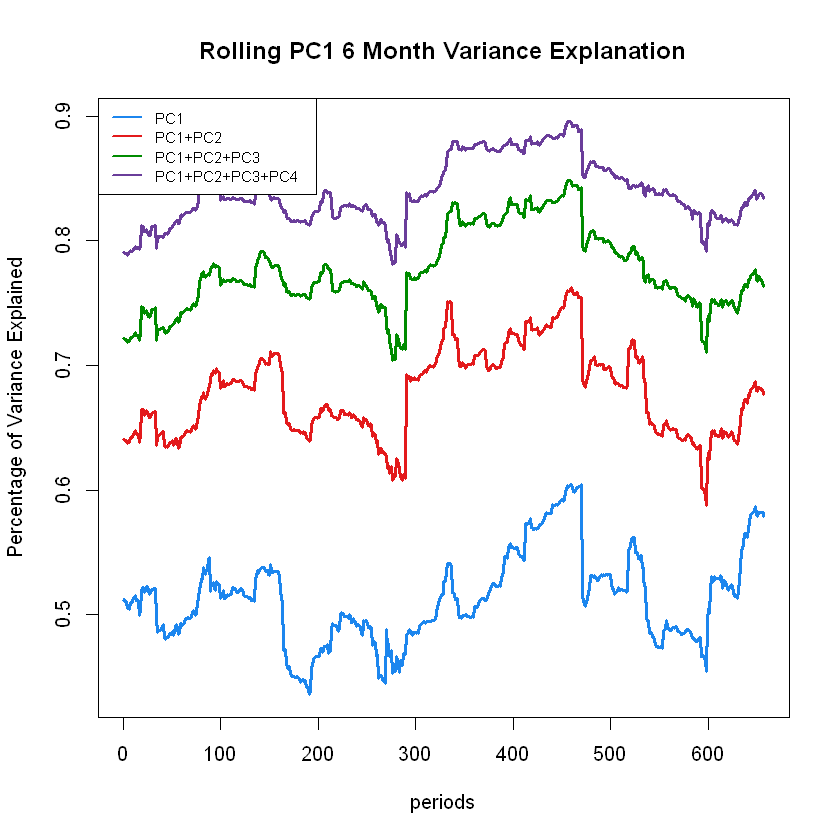
\includegraphics[width=0.6\textwidth]{PC1_6M.png}
\label{tech_6M_varexp}

\end{figure}

Looking at the 6-month variance explanation (Fig. \ref{tech_6M_varexp}) of PC1, we can see that our analysis seems relatively stable, even though the tech industry is fast-paced and turbulent. It shows that the variance explained by the top three or four PCA factors is consistently high and stable. In fact, it explains more than $70\%$ of the total variance of daily returns of the chosen stocks. It also agrees with the rolling 6-month PC1 and PC2 loadings illustrated above, because it manages to capture the instability of NVIDIA stock.


The following figures (Fig. \ref{3-6monthLoading}) show the weight coefficients for the stocks in the first three components that are obtained by applying PCA to the intervals of $k$ months (counting only business days) and these intervals are shifted by 1 day to compute the loadings for the all the days for which the data for next $k$ months is available. For $k=1$, the data is too noisy to be useful. However for the 6-month window the analysis seems relatively stable, except for around date 300 on the 6-month plot.
\\
 \newline

\begin{figure}[H]
\caption{}
\centering
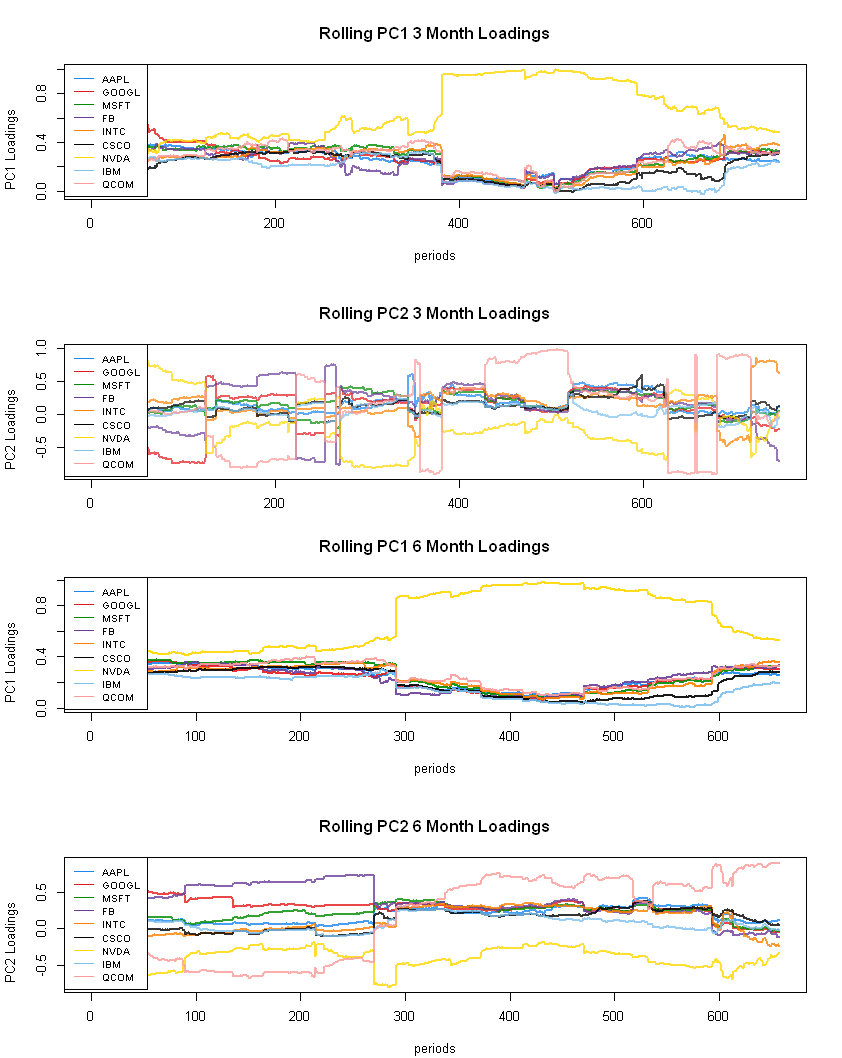
\includegraphics[width=0.7\textwidth]{36mload.png}
\label{3-6monthLoading}
\end{figure}


\subsection{Discussion of NVIDIA jump}

For both the variance-explanation and the loading graphs,  we observe that NVIDIA returns start to cause the majority of variance starting approximately x-point 300 of the 6-month graph and 400 of the 3-month graph. This is around 480 business days past the initial date in our dataset (1 of January, 2015), which corresponds roughly to November of 2016. 


When cross-checking our results with history of NVIDIA stock prices we discovered that this company indeed exhibited a significant increase in stock prices during November of 2016, following the release of the company's promising quarterly report (see Fig.\ref{news}). This jump in returns is much larger than that of any other of the companies we are looking at, which means it will be responsible for a larger amount of the total variance of the data.

\begin{figure}[H]
\caption{}
\centering

\includegraphics[width=0.8\textwidth]{Newspaper.png}
\label{news}
\end{figure}

This observation we made judging purely from PCA analysis shows that PCA is an effective tool for finding the stocks with the biggest relative variance in the historical data. 

\begin{figure}[h]
    \caption{}
    \centering
    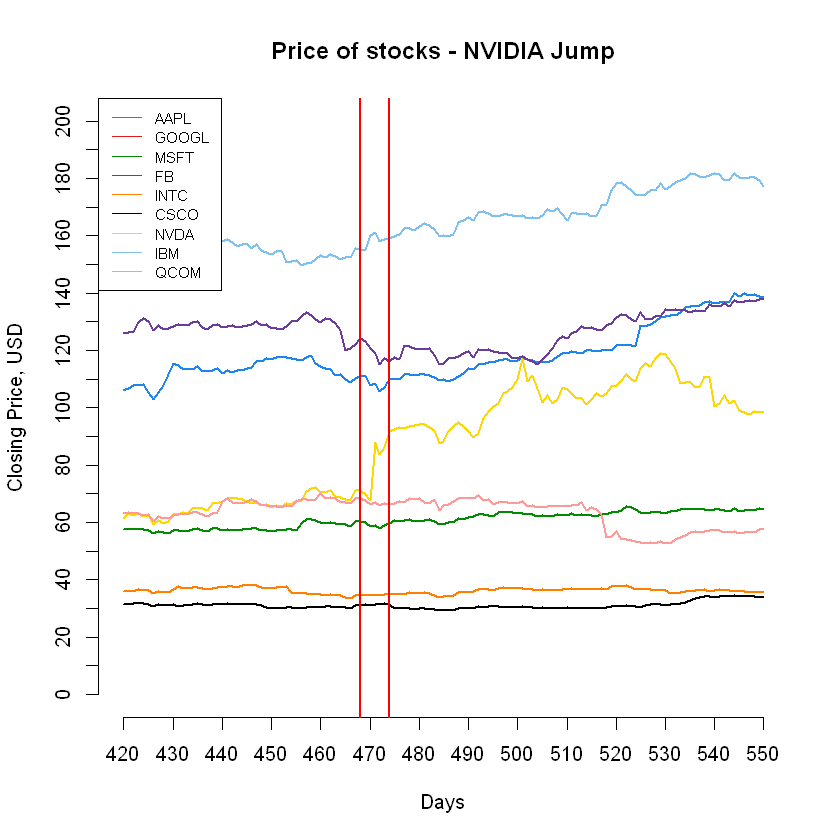
\includegraphics[width=0.7\textwidth]{nvidia_jump.png}
\end{figure}


\pagebreak
\section{Second Application - European Stock Market Indexes}

\subsection{Data Set}

For the second application, I used data from the prices of European stock market indexes. In particular, we are using  indexes from Belgium, France, Germany, Greece, Italy, Netherlands, Spain, UK, and Switzerland. The indexes used are: \texttt{BEL 20, CAC All Tradeable, GDAXI, ATHEX, FTSE MIB, AEX, IBEX 35, FTSE, and SSMI}. The data can be summarized in figure \ref{index_prices}.

\begin{figure}[H]
    \caption{}
    \centering
    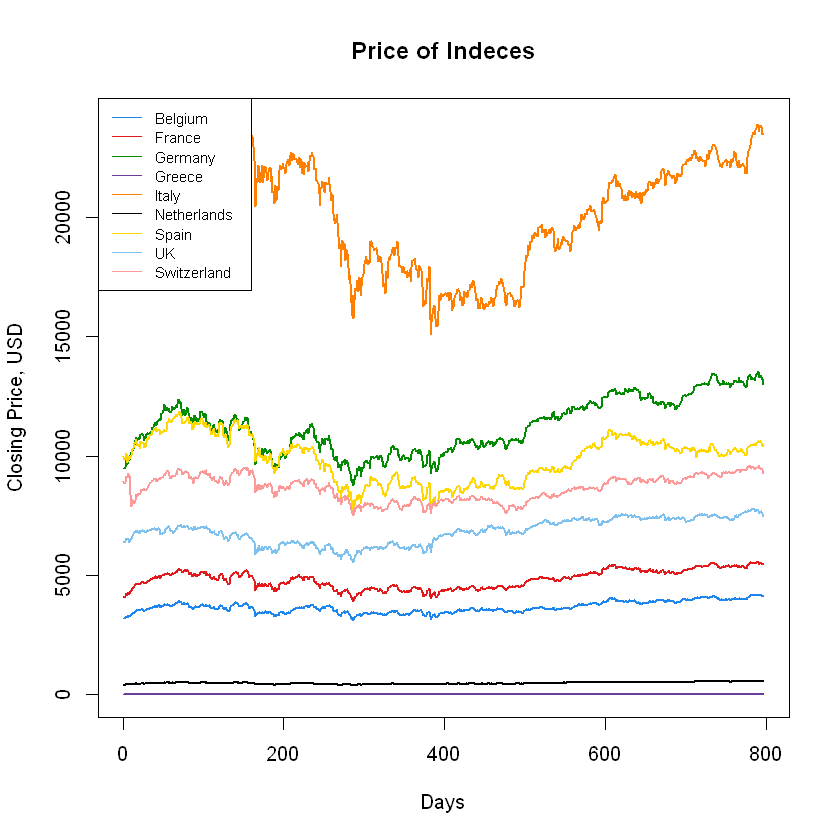
\includegraphics[width=0.75\textwidth]{index_prices.png}
    \label{index_prices}
\end{figure}

\subsection{Results}

After we apply the same method of preparing the data as explained in the previous application, and apply the principal component analysis, we get that our first principal component explains around 65\% and the second one around 27\% of the total variance. The variance explanation for each of the components can be viewed in figure \ref{indexvars}. This makes intuitive sense, since Greece is one of the most volatile countries here, so its price vs the others (as the loadings of PC2 show) would account for a large percentage of the total variance.

\begin{figure}[H]
    \caption{}
    \centering
    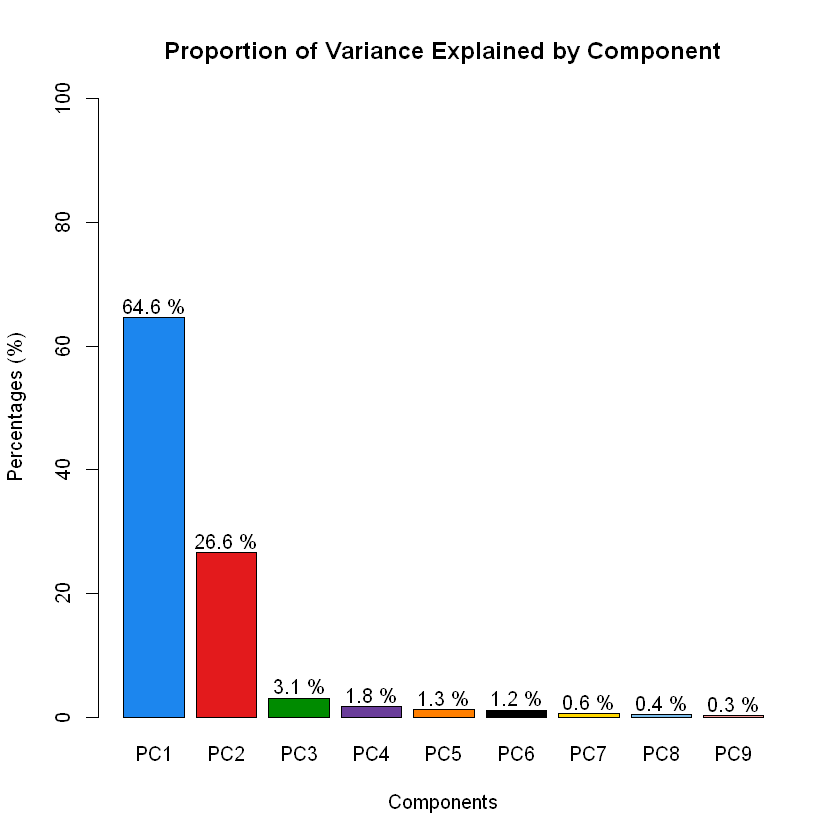
\includegraphics[width=0.7\textwidth]{index_variance.png}
    \label{indexvars}
\end{figure}

Furthermore, as seen in figure \ref{index_loadings}, the first principal component reflects the general market trend of the European countries, while the second one reflects how most countries are doing compared to Greece. The third principal component reflects how other countries are doing compared to Italy and Spain.

\begin{figure}[H]
    \caption{}
    \centering
    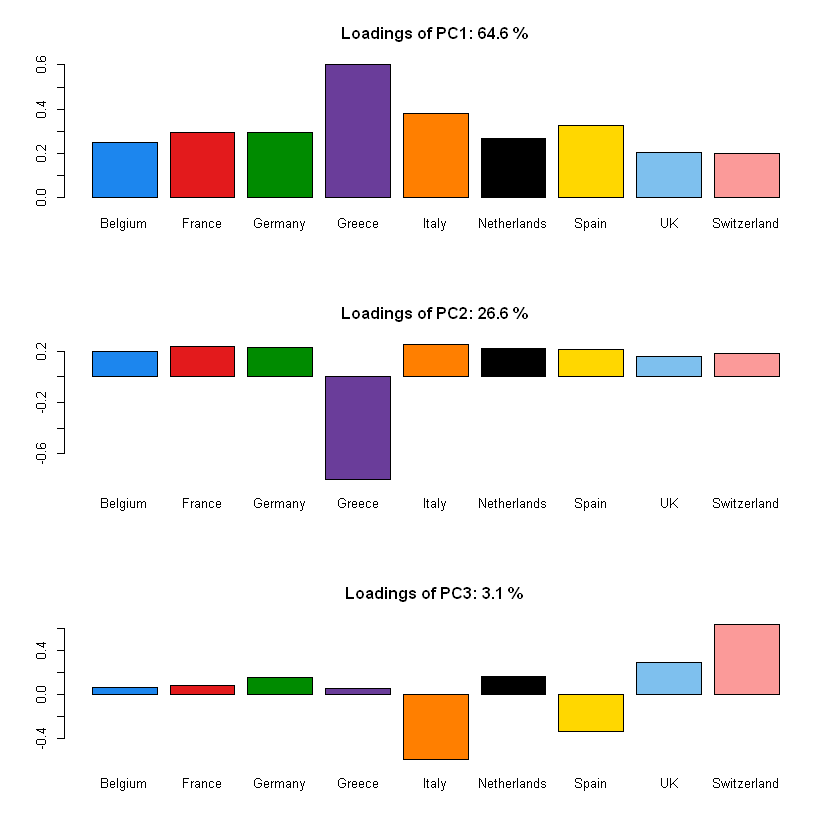
\includegraphics[width=0.7\textwidth]{index_loading1.png}
    \label{index_loadings}
\end{figure}


\subsection{Stability of Analysis}

Again, as shown in our 6-month rolling principal component analysis, the loadings (Fig. \ref{index-6m-loading}) and the percentage of variance (Fig. \ref{index-6m-var}) stay relatively constant. This means that our analysis is robust and indicative of the actual market.

\begin{figure}[H]
    \caption{}
    \centering
    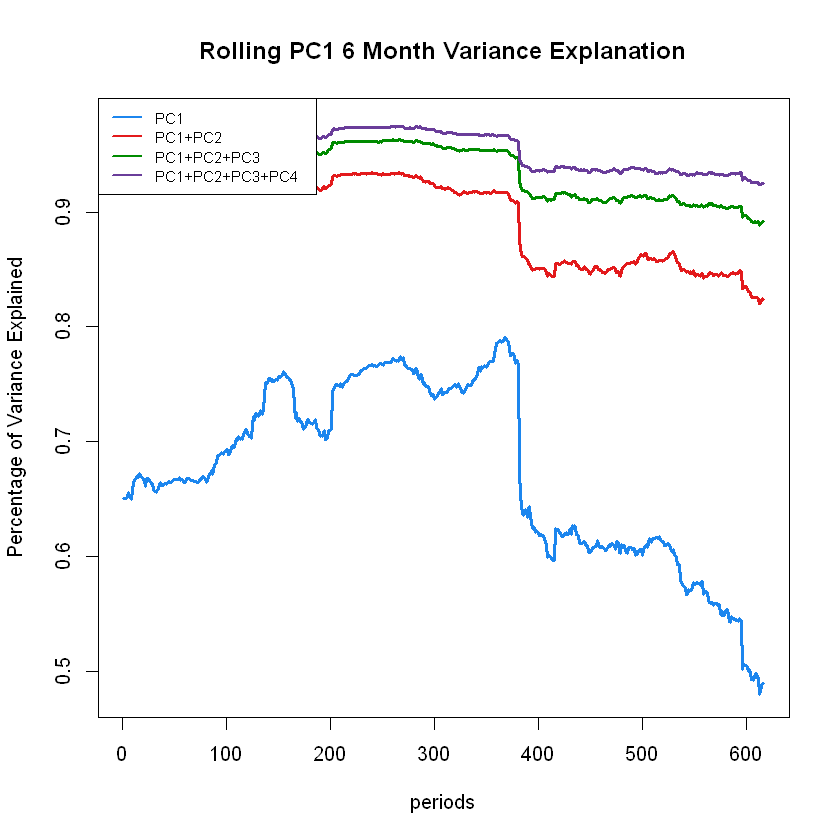
\includegraphics[width=0.7\textwidth]{index_6Mvar.png}
    \label{index-6m-var}
\end{figure}

\begin{figure}[H]
    \caption{}
    \centering
    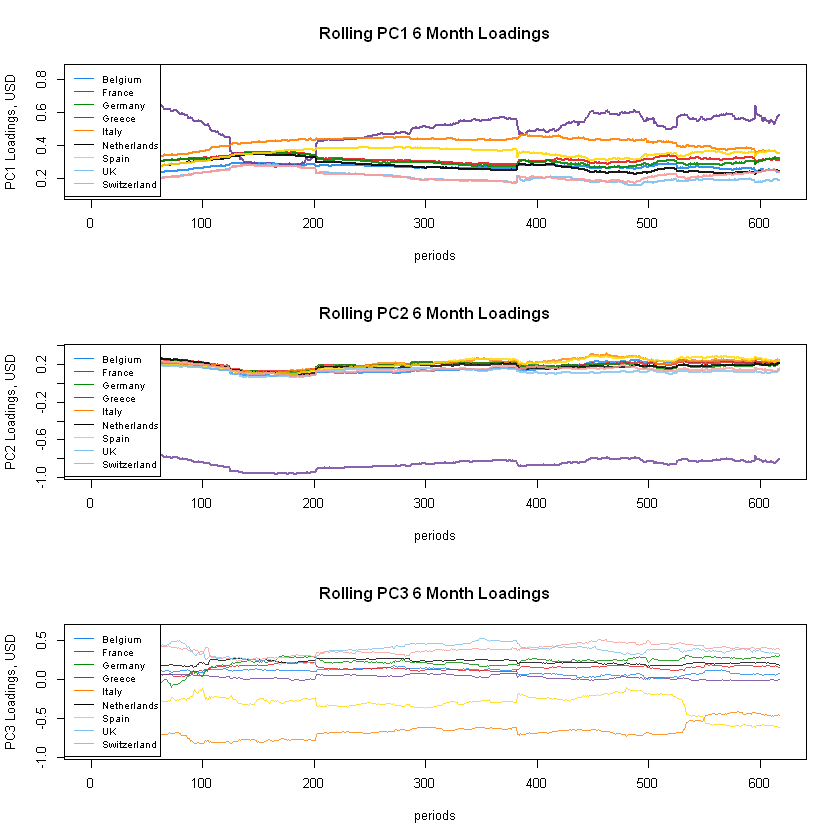
\includegraphics[width=0.7\textwidth]{index_6M_loading.png}
    \label{index-6m-loading}
\end{figure}

\section{PCA Portfolios}
A principal component portfolio is a basket of tradeable products where each one is weighted by the PC weight. For example, for the technology stock application, PC1 portfolio is expected to have the most of the variance, PC2 portfolio is expected to have the second largest variance, etc. In our first example, PC1 realization reflects the general trend across technology stocks, and PC2 reflects the divergence between the rest of the tech companies and NVIDIA. 

\begin{figure}[H]
    \caption{Technology Stocks}
    \centering
    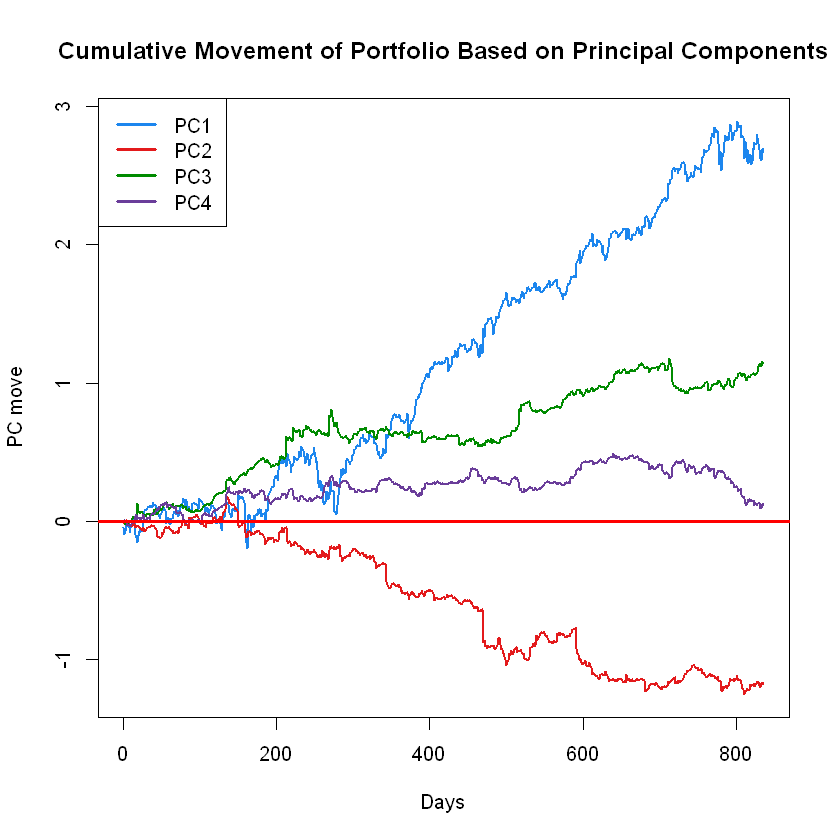
\includegraphics[width=0.7\textwidth]{PC_port.png}
    \label{tech_pcport}
\end{figure}



 
In figure \ref{tech_pcport} we can see the returns of the portfolios based on each of the first 4 principal components of the technology stocks example. It is obvious that the general trend of the tech industry is increasing, as shown by the realization of PC1 and that shorting a large amount of NVidia while buying stocks of the other companies reflected by PC2 would not be beneficial.
\\\par
In figure \ref{index_pcport} we can see the returns of the portfolios based on each of the first 4 principal components of the country index example. It is interesting to see that both betting on all the countries' indexes, as well as betting against Greece will be positive.

\begin{figure}[H]
    \caption{Country Indexes}
    \centering
    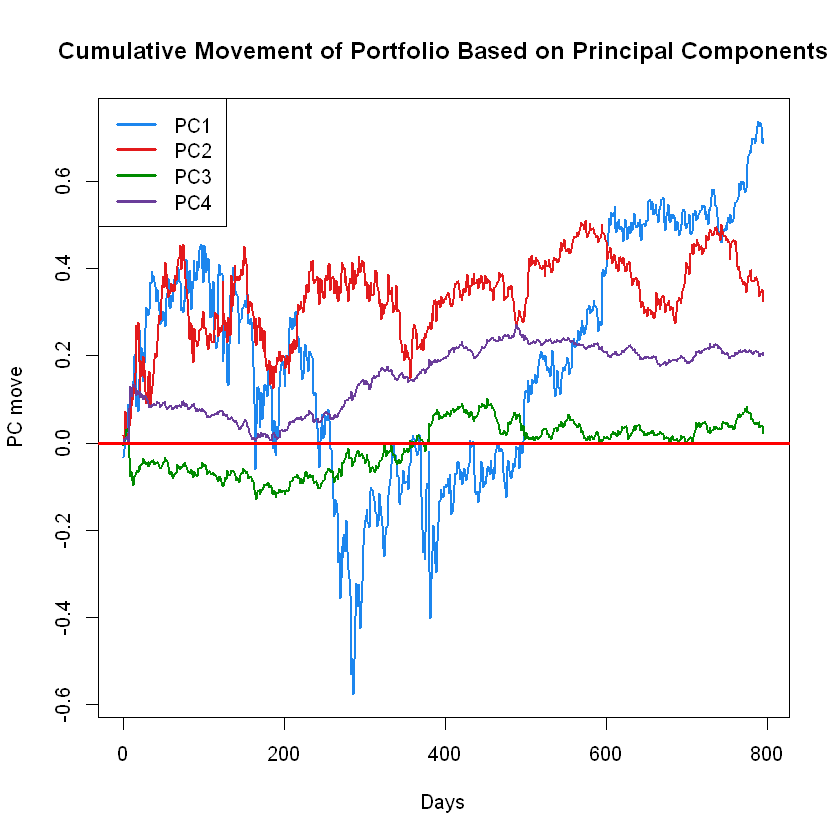
\includegraphics[width=0.7\textwidth]{index_PCport.png}
    \label{index_pcport}
\end{figure}

In general, the investment process usually blends a variety of strategies in an overall portfolio, seeking diversification. The resulting portfolio may have unintended overall exposure. PCA allows the investor to hedge volatile components that do not contribute to positive expected value.

Specifically, for a portfolio with weights $V$ across components, the exposure to the $n^{th}$ PC component is $Vu_{n}$. In order to eliminate exposure to the $k^{th}$ PC factor, we can construct $V'=V-(Vu_k)u_k$. The resulting portfolio will be PCk neutral. That is $V'u_k=0$. The variance of the resulting portfolio is $V'^{T}\Sigma V'$. If the expected value of $V$ and $V'$ are close to each other, the investor essentially preserves this expected value while reducing volatility.





\section{Conclusion}
After looking into the method of Principal Component Analysis and adequately preparing the data, we perform PCA on two different datasets. We find that the first principal component of PCA does indeed account for the most of the total variance in both examples, dropping off dramatically with each PC. This makes sense in context, considering that the stocks chosen are not entirely independent of each other. Our example, when applied to a wider time window, illustrates the stability of the method as well. We can conclude, based on our example of tech company stocks, that PCA proves to be a useful and valuable tool in data analysis as well as discuss its use in portfolio optimization. 


\end{document}
